\documentclass{beamer}
\usepackage{subfigure}
\usepackage[latin1]{inputenc}
\usepackage{braket}
\usepackage{caption}
\usepackage{amsmath,amssymb,amsthm}
\input{qcircuit}

\usetheme{Warsaw}
\title[What's the deal with QC]{What's the deal with Quantum Computing\\-How to break RSA-}
\author{Maksim Levental}
%\institute{Math-linux.com}
\date{\today}
\begin{document}
\bibliographystyle{acm}
\setbeamertemplate{caption}{\raggedright\insertcaption\par}
\begin{frame}
\titlepage
\end{frame}


\begin{frame}{Recap}
  
\begin{itemize}
     \item A single qubit is a (unit length) linear combination of the basis vectors $\Ket{0},\Ket{1}$
  
       \[
       \psi=\alpha\Ket{0}+\beta\Ket{1}
       \] 
         
     \item Measurement $\iff$ non-deterministic wave function collapse $\iff$ all 
information lost
     \item Unitary transformations correspond to gates. 1-qubit gates are matrices 
       \[
       H=\frac{1}{\sqrt{2}}\begin{pmatrix}1 & 1\\
         1 & -1
       \end{pmatrix}
       \]

       \item $n$-qubit systems (registers) are represented by vectors (tensors) in the 
         tensor product of the vector spaces that each of the individual qubits are 
         elements of
\end{itemize}
\end{frame}

\begin{frame}{Recap}
\begin{itemize}
  \item[] 
    \begin{eqnarray*}
    \left(\frac{1}{\sqrt{2}}\left(\Ket{0}+\Ket{1}\right)\right)\otimes\left(\frac{1}{\sqrt{2}}\left(\Ket{0}+\Ket{1}\right)\right) &=&  \frac{1}{2}\bigg(\Ket{0}\Ket{0}+\Ket{0}\Ket{1}+\\
    &&\Ket{1}\Ket{0}+\Ket{1}\Ket{1}\bigg)
    \end{eqnarray*}
  \item Gates on single qubit systems also map to ``$n$-gates'' on $n$-qubit systems (entrywise)
    \begin{eqnarray*}
      H^{\otimes 2}\Ket{0}\Ket{0} & = & \left(H\Ket{0}\right)\otimes\left(H\Ket{0}\right)\\
                               & = & \left(\frac{1}{\sqrt{2}}\left(\Ket{0}+\Ket{1}\right)\right)\otimes\left(\frac{1}{\sqrt{2}}\left(\Ket{0}+\Ket{1}\right)\right)\\  
    \end{eqnarray*}
  \item Entangled states are important: for $\psi \in V\otimes W$ there \textbf{do not exist} $\phi \in V$ and $\varphi \in W$ such that
    \[
     \psi=\frac{\Ket{0}\Ket{0}+\Ket{1}\Ket{1}}{\sqrt{2}}=\phi\otimes\varphi
    \]
\end{itemize}
\end{frame}

%\begin{frame}{Bloch Sphere}
%\begin{figure}[ht]
%  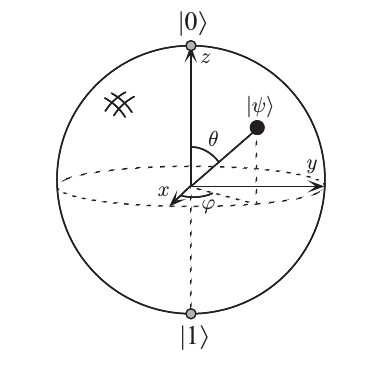
\includegraphics[scale=0.55]{pasted12}
%\end{figure}
%\[
%\Ket{\psi}=\cos\left(\frac{\theta}{2}\right)\Ket{0}+e^{i\varphi}\sin\left(\frac{\theta}{2}\right)\Ket{1}
%\]
%\end{frame}



\begin{frame}{Deutsch's Problem}
``Reversible computation without can be done \textbf{efficiently}, without the production of garbage bits whose values depend on the input to the computation. That is, if there is an irreversible circuit computing a function $f$, then there is an efficient simulation of this circuit by a reversible [unitary transformation/quantum] circuit with action''\cite{Nielsen:2011:QCQ:1972505}
\[
\Ket{x}\Ket{y}\to\Ket{x}\Ket{y\oplus f\left(x\right)}
\]

\end{frame}


\begin{frame}{Deutsch's Problem}

Let $f\left(x\right):\left\{ 0,1\right\} \to\left\{ 0,1\right\}$ and suppose we are guaranteed that $f$ is either balanced (1 on half of its domain and 0 on the other half)
or constant (1 or 0 on the entire domain). How many evaluations classically to discriminate? ``Quantumly'' you only need
to evaluate $f$ once! Let $U_f$ be the quantum circuit such that 
\[
U_f\Ket{x}\Ket{y}=\Ket{x}\Ket{y\oplus f\left(x\right)}
\]
With some algebra (keeping in mind the small-ish domain and range of $f$)

\[
U_{f}\left(\Ket{x}\left(\frac{\Ket{0}-\Ket{1}}{\sqrt{2}}\right)\right)=\left(-1\right)^{f\left(x\right)}\Ket{x}\left(\frac{\Ket{0}-\Ket{1}}{\sqrt{2}}\right)
\]
\end{frame}


\begin{frame}{Deutsch's Algorithm}
Construct the quantum circuit
\begin{figure}[ht]
  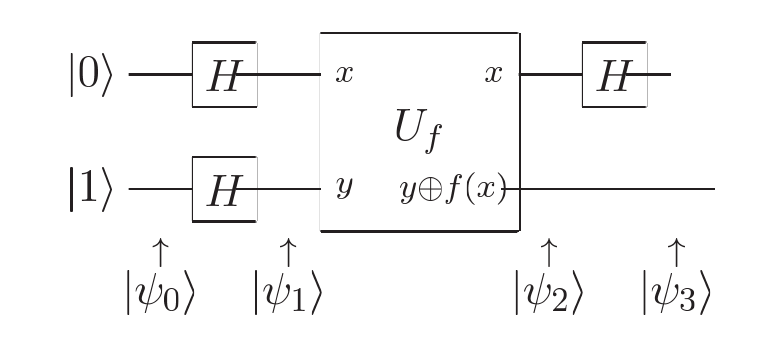
\includegraphics[scale=0.33]{pasted1}
\end{figure}
\[
\Ket{\psi_{1}} = H^{\otimes2}\left(\Ket{0}\otimes\Ket{1}\right)
\]

\[
\psi_{2}=U_{f}\Ket{\psi_{1}}=\begin{cases}
\pm & \left(\frac{\Ket{0}+\Ket{1}}{\sqrt{2}}\right)\left(\frac{\Ket{0}-\Ket{1}}{\sqrt{2}}\right)\text{ if }f\left(0\right)=f\left(1\right)\\
\pm & \left(\frac{\Ket{0}-\Ket{1}}{\sqrt{2}}\right)\left(\frac{\Ket{0}-\Ket{1}}{\sqrt{2}}\right)\text{ if }f\left(0\right)\neq f\left(1\right)
\end{cases}
\]

\end{frame}


\begin{frame}{Deutsch's Algorithm}

The final Hadamard gate on the first qubit gives
\[
\psi_{3}=\begin{cases}
\pm & \Ket{0}\left(\frac{\Ket{0}-\Ket{1}}{\sqrt{2}}\right)\text{ if }f\left(0\right)=f\left(1\right)\\
\pm & \Ket{1}\left(\frac{\Ket{0}-\Ket{1}}{\sqrt{2}}\right)\text{ if }f\left(0\right)\neq f\left(1\right)
\end{cases}
\]

Now if we measure the first qubit we know whether $f\left(0\right)=f\left(1\right)$
or $f\left(0\right)\neq f\left(1\right)$ (depending on whether we get $\Ket{0}$ or $\Ket{1}$ ). Succinctly stated this allows us to measure a global property: since $f\left(0\right)\oplus f\left(1\right)=0$ if $f\left(0\right)=f\left(1\right)$ and 1 otherwise
\[
\psi_{3}=\pm\Ket{f\left(0\right)\oplus f\left(1\right)}\left(\frac{\Ket{0}-\Ket{1}}{\sqrt{2}}\right)
\] 

Naive interpretation is that this is a randomized algorithm but in truth interference effects (the final Hadmard gate)
are used to discern global properties ($H$ is a generalized DFT).
 

\end{frame}

\begin{frame}{Deutsch-Jozsa Algorithm}

Generalize to $f\left(x\right):\left\{ 0,1\right\} ^{n}\to\left\{ 0,1\right\} $ and still $f$ is either balanced or constant.
How many evaluations classically? $2^{n-1}+1$ but quantumly still 1!
 
\begin{figure}[ht]
  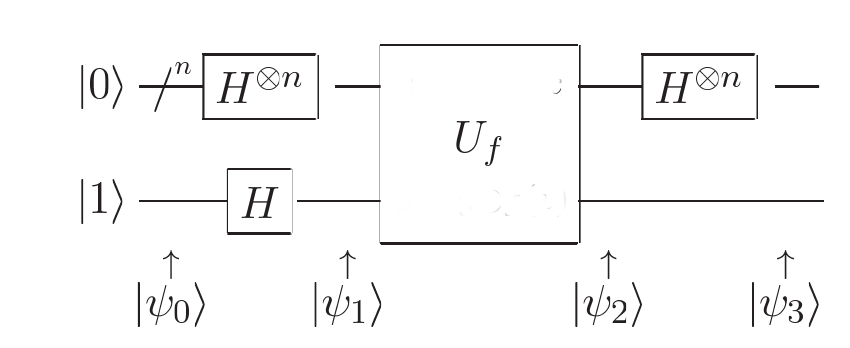
\includegraphics[scale=0.33]{pasted2}
\end{figure}

\[
\psi_{0}=\Ket{0}^{\otimes n}\Ket{1}
\]
 then 
\[
\psi_{1}=\sum_{x\in\left\{ 0,1\right\} ^{n}}\frac{\Ket{x}}{\sqrt{2^{n}}}\left(\frac{\Ket{0}-\Ket{1}}{\sqrt{2}}\right)
\]

\end{frame}

\begin{frame}{Deutsch-Jozsa Algorithm}
The first register is a superposition of all basis states in the $n$-qubit
computational basis. Using the simplification above again we have
that 
\[
\psi_{2}=U_{f}\psi_{1}=\sum_{x\in\left\{ 0,1\right\} ^{n}}\frac{\left(-1\right)^{f\left(x\right)}\Ket{x}}{\sqrt{2^{n}}}\left(\frac{\Ket{0}-\Ket{1}}{\sqrt{2}}\right)
\]
and the last Hadamard operator 
\[
\psi_{3}=H^{\otimes n}\psi_{2}=\sum_{z\in\left\{ 0,1\right\} ^{n}}\sum_{x\in\left\{ 0,1\right\} ^{n}}\frac{\left(-1\right)^{x\cdot z+f\left(x\right)}\Ket{x}}{2^{n}}\left(\frac{\Ket{0}-\Ket{1}}{\sqrt{2}}\right)
\]
where $x\cdot z$ is bitwise inner product mod 2.  
\end{frame}

\begin{frame}{Deutsch-Jozsa Algorithm}
Let's observe the
top register (query register). Note that the amplitude for $\Ket{0}^{\otimes n}$
is $\sum_{x}\left(-1\right)^{f\left(x\right)}/2^{n}$. If $f$ is
constant then
\[
\sum_{x\in\left\{ 0,1\right\} ^{n}}\frac{\left(-1\right)^{f\left(x\right)}}{2^{n}}=\pm1
\]
and because $\psi_{3}$ must be unit length we will certainly measure
$\psi_{3}$ to be in the $\Ket{0}^{\otimes n}$ state. If $f$ is
balanced then by definition of balanced ($f\left(x\right)$ will be
even as often as odd) 
\[
\sum_{x\in\left\{ 0,1\right\} ^{n}}\frac{\left(-1\right)^{f\left(x\right)}}{2^{n}}=0
\]
and we will certainly measure something other than $\Ket{0}^{\otimes n}$.
\end{frame}


\begin{frame}{Factoring integers - reduction to order finding}
Pick $x<N$. If $x$ and $N$ have a common factor then $\gcd(x,N)$ can be computed classically in polynomial time using Euclid's algorithm. Otherwise compute the order of $x$; the least $r$ such that
\[
x^r\equiv 1 \mod N
\]

With probability $p>1-\left(\frac{1}{2}\right)^q$, where $q$ is the number of prime factors in $N$, the order of $x$ will be even. Then
\[
x^r-1\equiv \left(x^{r/2}-1\right)\left(x^{r/2}+1\right)\equiv 0 \mod N
\]

and hence $N$ divides $\left(x^{r/2}-1\right)\left(x^{r/2}+1\right)$. If $1<x^{r/2}<N-1$ then 

\[
0<\left(x^{r/2}-1\right)<\left(x^{r/2}+1\right)<N
\]

and hence $\left(x^{r/2}-1\right),\left(x^{r/2}+1\right)$ must each have a factor of $N$. Compute $\gcd(x^{r/2}-1,N)$ and $\gcd(x^{r/2}+1,N)$ 

\end{frame}

\begin{frame}{Order example}
For $N=2013$ it's the case that $8^{20}\equiv 1 \mod N \iff 8^{20}- 1 \equiv 0 \mod N$ and 

\[
\left(8^{\frac{20}{2}}-1\right)\left(8^{\frac{20}{2}}+1\right)\equiv 0 \mod N
\]

But $\left(8^{\frac{20}{2}}-1\right)\equiv 1584 \mod N$ and  $\left(8^{\frac{20}{2}}+1\right)\equiv 1586 \mod N$ and $0<1584<1586<2013$ so 
\[
\gcd \left(1584,2013\right)=33 \qquad \gcd \left(1586,2013\right)=61
\]
 and $61\times 33=2013$

\end{frame}

\begin{frame}{Shor's Algorithm}

\begin{figure}[ht]
  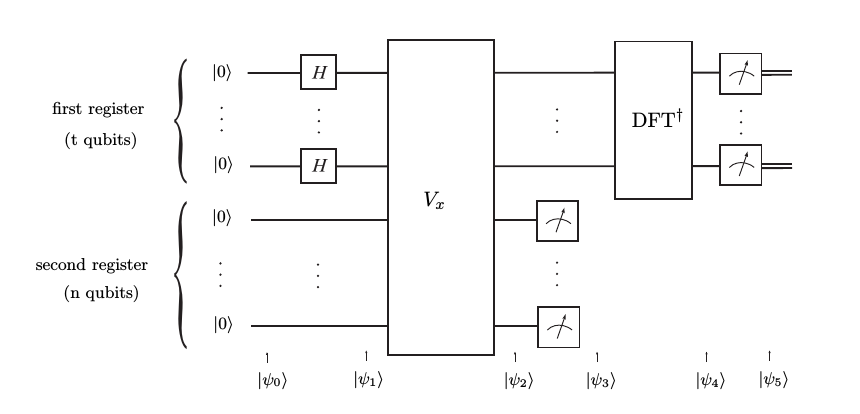
\includegraphics[scale=0.4]{pasted5}
\end{figure}

where 
\[
V_x \left(\ket{j}\ket{k}\right) = \ket{j}\ket{k+x^j}
\]

and

\[
DFT\left(\ket{k}\right) = \frac{1}{\sqrt{N}}\sum_{j=0}^{N-1}e^{2\pi i j k/N}\ket{j}
\]
\end{frame}

\begin{frame}{Shor's Algorithm}

Then
{\small

\[
\ket{\psi_2}=\frac{1}{\sqrt{2^t}}\sum_{j=0}^{2^t-1}\ket{j}\ket{x^j} \underset{r|2^t}{=} \frac{1}{\sqrt{2^t}}\sum_{b=0}^{r-1}\sum_{a=0}^{\frac{2^t}{r}-1}\ket{ar+b}\ket{x^b}
\]
}
\begin{figure}[ht]
  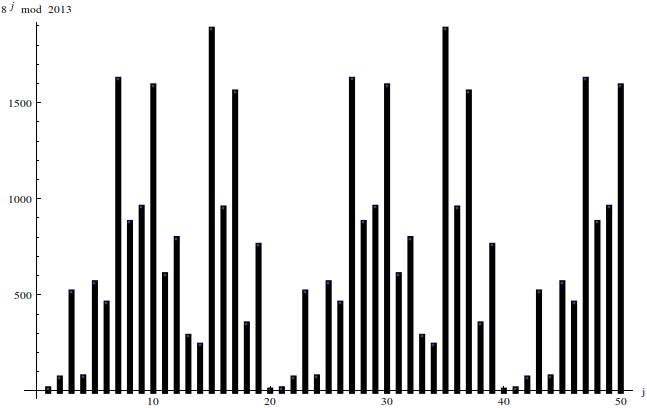
\includegraphics[scale=.3]{pasted9}
\end{figure}
\end{frame}
\begin{frame}{Shor's Algorithm}

\[
\ket{\psi_3}=\sqrt{\frac{r}{2^t}}\sum_{a=0}^{\frac{2^t}{r}-1}\ket{ar+b_0}\ket{x^{b_0}}
\]

\begin{figure}[ht]
  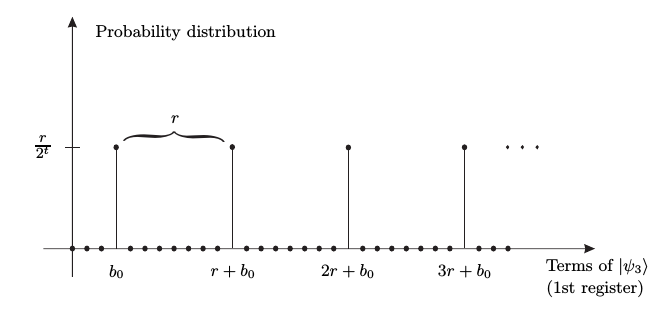
\includegraphics[scale=.5]{pasted7}
\end{figure}

\end{frame}
\begin{frame}{Shor's Algorithm}




{\small

\[
\ket{\psi_4}=\frac{1}{\sqrt{r}}\sum_{k=0}^{r-1}e^{2\pi \frac{k}{r}b_0}\ket{\frac{k2^t}{r}}\ket{x^{b_0}}
\]

Assuming the order of $x$, $r$ is a multiple of 2 (can be generalized), after measuring the first register we have $\ket{\psi_5}=\ket{\frac{k_0 2^t}{r}}$

\begin{figure}[ht]
  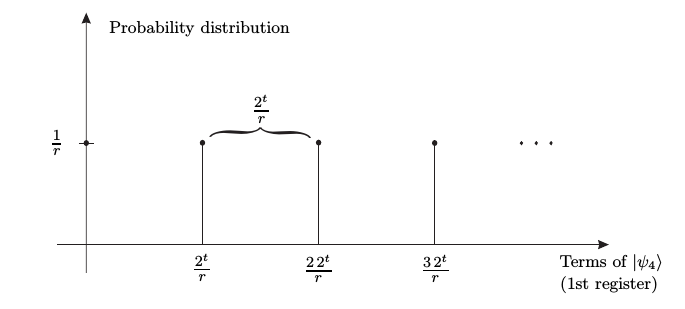
\includegraphics[scale=.45]{pasted6}
\end{figure}

If $k_0=0$ then we rerun. Otherwise divide $k_02^t/r$  by $2^t$. If $k_0,r$ are coprime then we can just take the denominator of $k_0/r$. Otherwise $r=r_1 r_2$ and we can find the order of $x^{r_1}$ to find $r$.
}
\end{frame}


\begin{frame}{Shor's Algorithm Implementation}
  
\begin{figure}[ht]
%\centering
    \begin{minipage}{0.15\linewidth}
       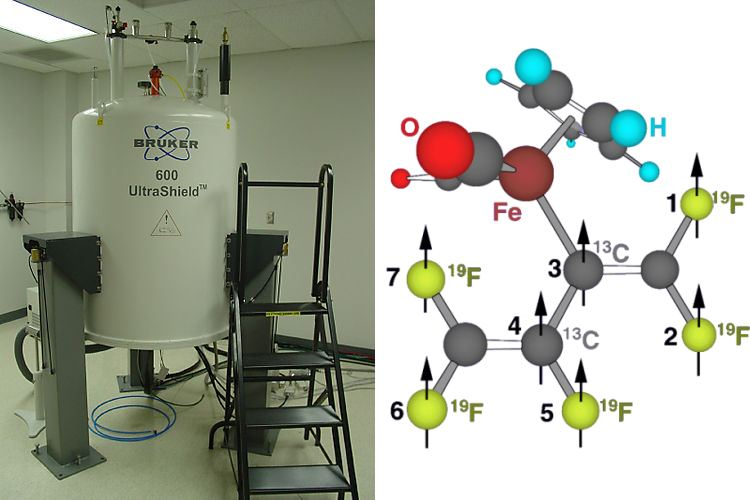
\includegraphics[scale=.2]{pasted10}
    \end{minipage}
    \qquad\qquad\qquad\qquad\qquad
    \begin{minipage}{0.2\linewidth}
       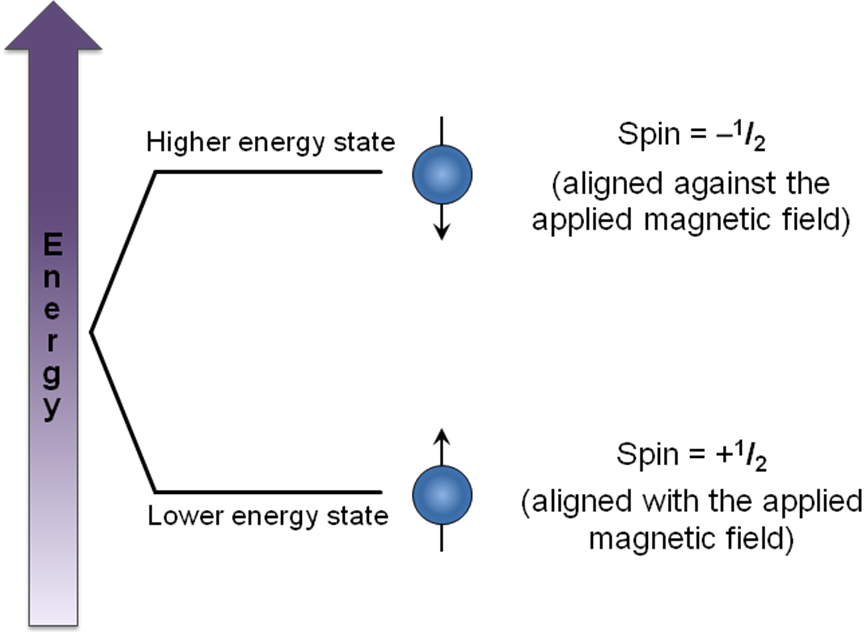
\includegraphics[scale=.3]{pasted11}
    \end{minipage}
\caption{Experimental realization of Shor's quantum factoring algorithm using nuclear magnetic resonance \cite{2001Natur.414..883V} }
\end{figure}
\end{frame}

\begin{frame}{Computability}

\begin{figure}[ht]
%\centering
{\small
    \begin{minipage}{0.4\textwidth}
       A \textbf{Probabilistic Turing machine} $M$ over an alphabet $A$ is $\left(Q,A,\delta,q_0,q_a,q_r\right)$ where
       \begin{itemize}
         \item $Q$ is the set of internal control states
         \item $q_0,q_a,q_r\in Q$ are initial,accepting, and rejecting states
         \item $\delta:Q\times A\times Q\times A\times\{-1,0,1\}\mapsto [0,1]$ is a transition probability function i.e.
           \[
             \sum_{\left(q_2,a_2,d\right)}\delta\left(q_1,a_1,q_2,a_2\right)=1
           \]
       \end{itemize}
    \end{minipage}
    \qquad
    \begin{minipage}{0.4\textwidth}
       A \textbf{Quantum Turing machine} $M$ over an alphabet $A$ is $\left(Q,A,\delta,q_0,q_a,q_r\right)$ where
       \begin{itemize}
         \item $Q$ is the set of internal control states
         \item $q_0,q_a,q_r\in Q$ are initial,accepting, and rejecting states
         \item $\delta:Q\times A\times Q\times A\times\{-1,0,1\}\mapsto \mathbb{C}$ is a transition probability function i.e.
           \[
             \sum_{\left(q_2,a_2,d\right)}|\delta\left(q_1,a_1,q_2,a_2\right)|^2=1
           \]
       \end{itemize}
    \end{minipage}
}
\end{figure}

\end{frame}

\begin{frame}{Computability Theorems}
  \begin{itemize}
    \item $\textbf{BPP}\subset \textbf{BQP}$
    \item A language $L$ has uniformly polynomial circuits iff $L\in \textbf{P}=\bigcup_k \textbf{TIME}\left( n^k \right)$
    \item All Boolean circuits can be simulated using reversible Boolean circuits
  \end{itemize}

\begin{figure}[ht]
\tiny
\centering
    \begin{minipage}{.5\linewidth}
       \Qcircuit @C=1em @!R {
         \lstick{\Ket{x}}   &   \qw   &   \ctrl{1}   &   \qw   &   \rstick{\Ket{x}}   \qw                     \\
         \lstick{\Ket{y}}   &   \qw   &   \ctrl{1}   &   \qw   &   \rstick{\Ket{y}}   \qw                     \\
         \lstick{\Ket{z}}   &   \qw   &   \targ      &   \qw   &   \rstick{\Ket{x \oplus (y \wedge z})} \qw
       }
    \end{minipage}%
    \qquad\qquad\qquad
    \begin{minipage}{0.5\linewidth}
      \[
      \begin{bmatrix}1 & 0 & 0 & 0 & 0 & 0 & 0 & 0 \\0 & 1 & 0 & 0 & 0 & 0 & 0 & 0 \\0 & 0 & 1 & 0 & 0 & 0 & 0 & 0 \\0 & 0 & 0 & 1 & 0 & 0 & 0 & 0 \\0 & 0 & 0 & 0 & 1 & 0 & 0 & 0 \\0 & 0 & 0 & 0 & 0 & 1 & 0 & 0 \\0 & 0 & 0 & 0 & 0 & 0 & 0 & 1 \\0 & 0 & 0 & 0 & 0 & 0 & 1 & 0 \\\end{bmatrix}
      \]
    \end{minipage}
\caption{Toffoli gate}
\end{figure}
\begin{itemize}
\item Toffoli is classically universal but not quantum universal, but $\{TOF,H\}$ are quantum universal and both have successfully implemented \cite{5558424,2009PhRvL.102d0501M}. 
\end{itemize}
\end{frame}


\begin{frame}{Simon's problem and complexity results}
Let $f\left(x\right):\left\{ 0,1\right\} ^{n}\to\left\{ 0,1\right\}^n$ and we are guaranteed that $\exists ~ s\in \{0,1\}^n$ such that 
\[
  f\left(y\right)=f\left(z\right) \iff \left(y=z \vee y\oplus z = s\right)
\]

Find $s$. Classically $\Omega\left(2^{n/2}\right)$ while quantumly $O\left(n\right)$. Also quantumly optimal; any quantum algorithm
needs to make $\Omega\left(n\right)$. 

\vspace{\baselineskip}

Yields an oracle separation between \textbf{BPP} and \textbf{BQP}. 

\vspace{\baselineskip}



Deutsch-Josza only yields a separation between \textbf{P} and \textbf{EQP}

\end{frame}
\begin{frame}{More EQP}
Let $f\left(x\right):\left\{ 0,1\right\} ^{n}\to\left\{ 0,1\right\}$ be the PARITY function. Classically how many operations must be performed for $f$ to be computed?
Quantumly only $n/2$ queries to the bit string need to be made \cite{de2002quantum}.  

\vspace{\baselineskip}

Compute the ``square-free'' part of an integer $N$, i.e. $r$ such that
\[
N=r\cdot s^2
\]

No known polynomial time classical algorithm; ``almost'' as hard as factorization itself \cite{Okamoto98anew}. Quantumly in $O\left(\left(\log \log N\right)^2\right)$ \cite{li2012efficient}. 

\vspace{\baselineskip}


Interestingly while this algorithm uses the Fourier transform it is exact (as opposed to Shor's).

\end{frame}

\begin{frame}{D-Wave}
\begin{figure}
  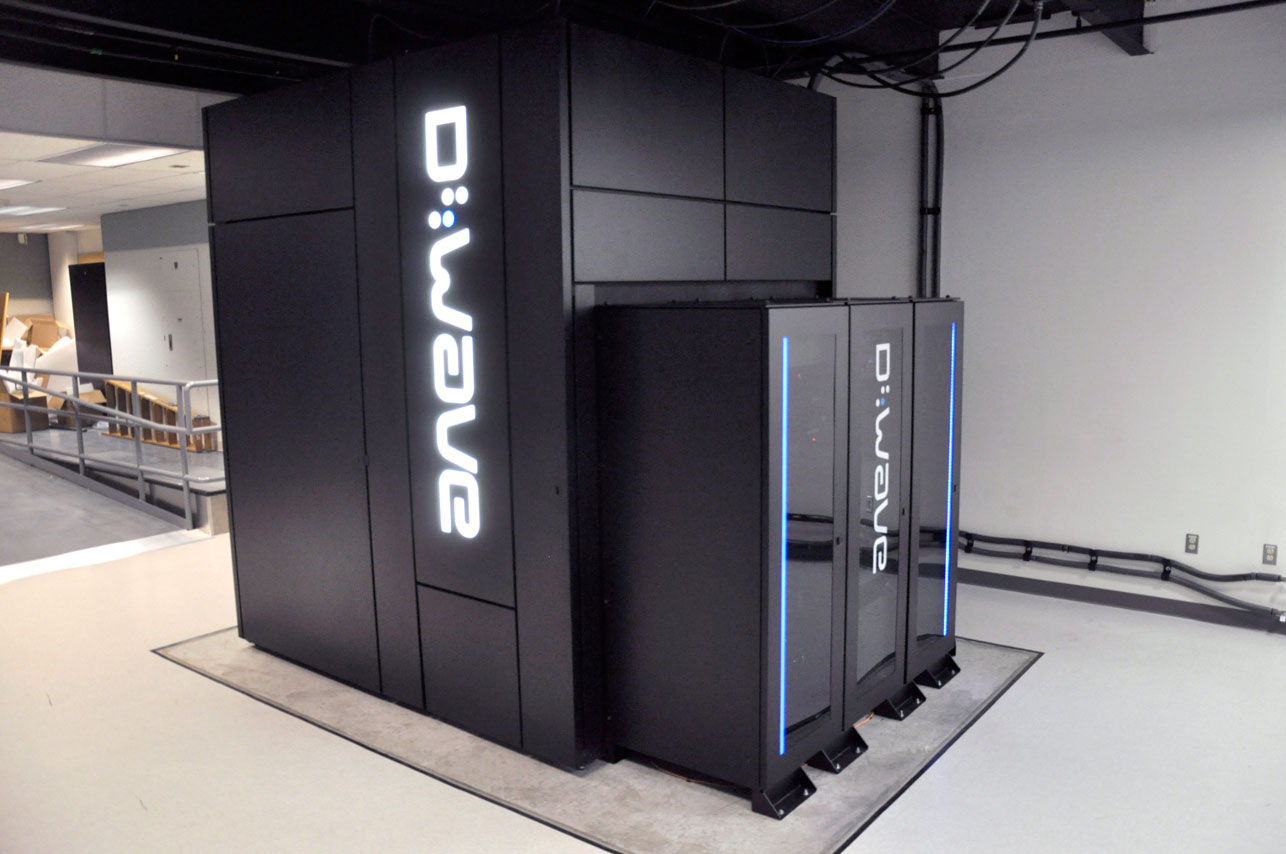
\includegraphics[scale=.25]{pasted14}
\end{figure}
\end{frame}


\begin{frame}{D-Wave}

\begin{figure}[ht]
\tiny
\centering
    \begin{minipage}{.2\linewidth}
      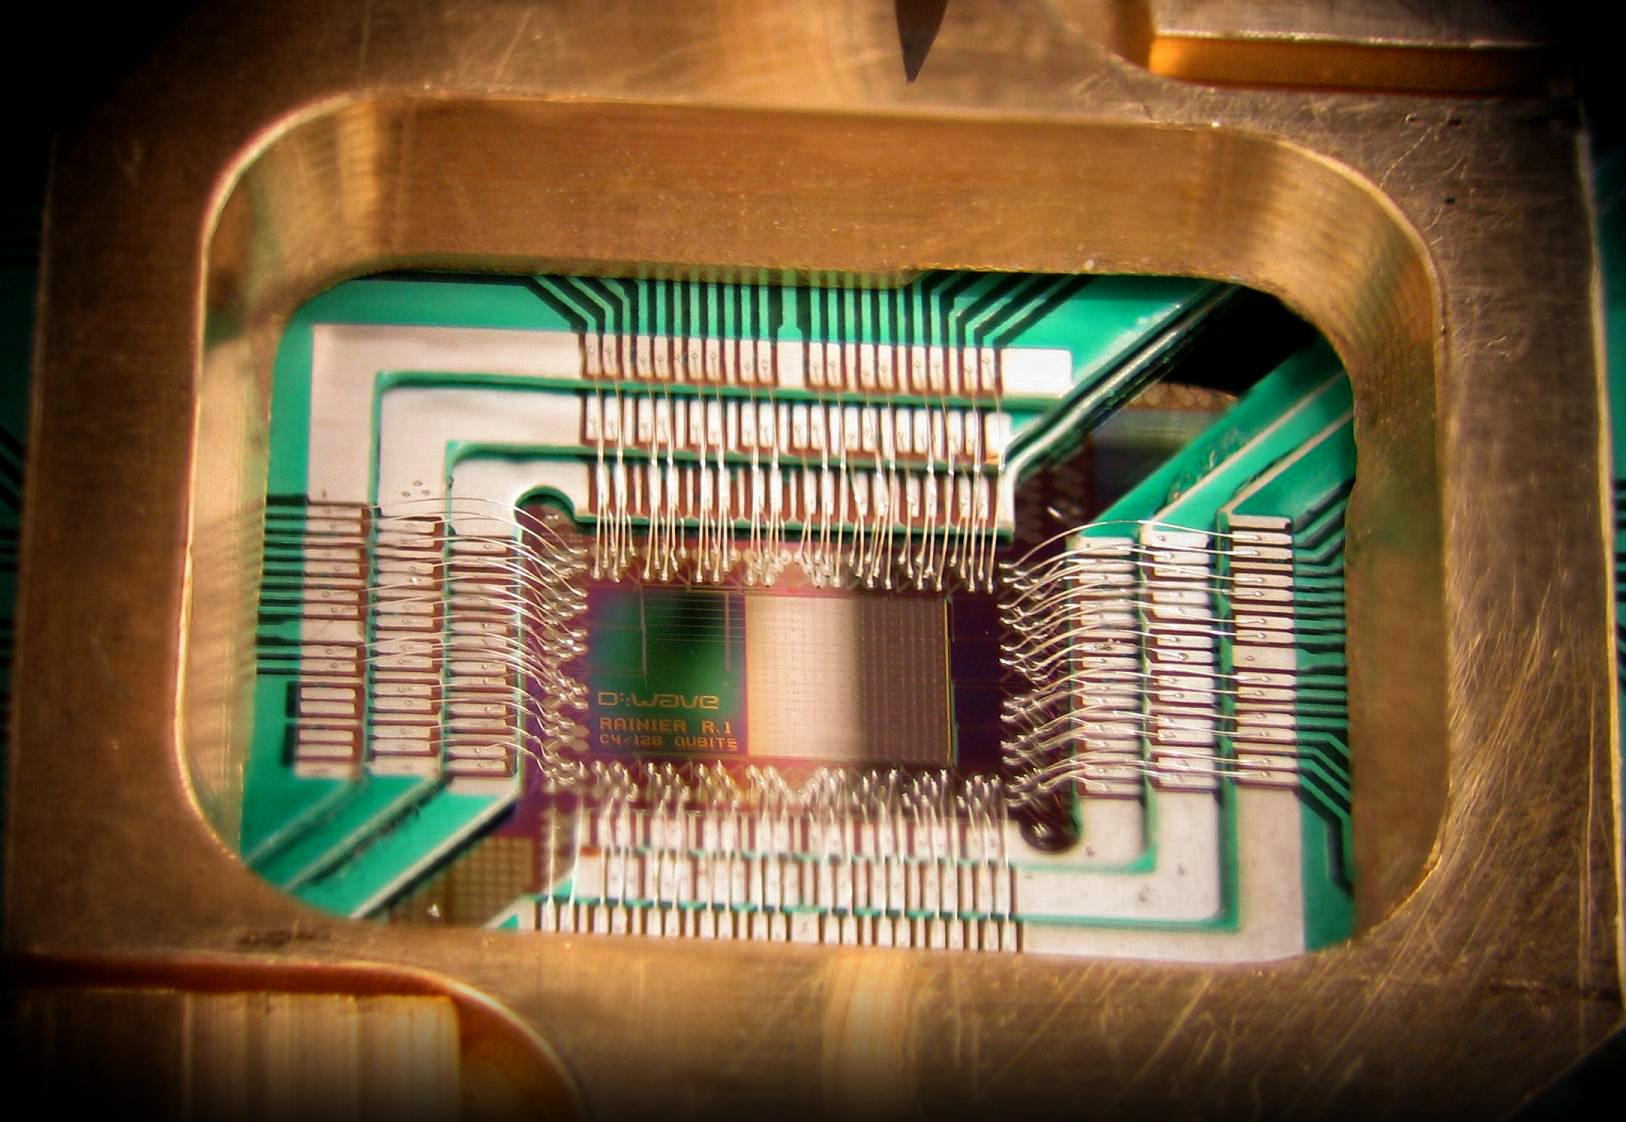
\includegraphics[scale=.15]{pasted13}
    \end{minipage}%
    \qquad\qquad\qquad\qquad\qquad\qquad
    \begin{minipage}{.5\linewidth}
      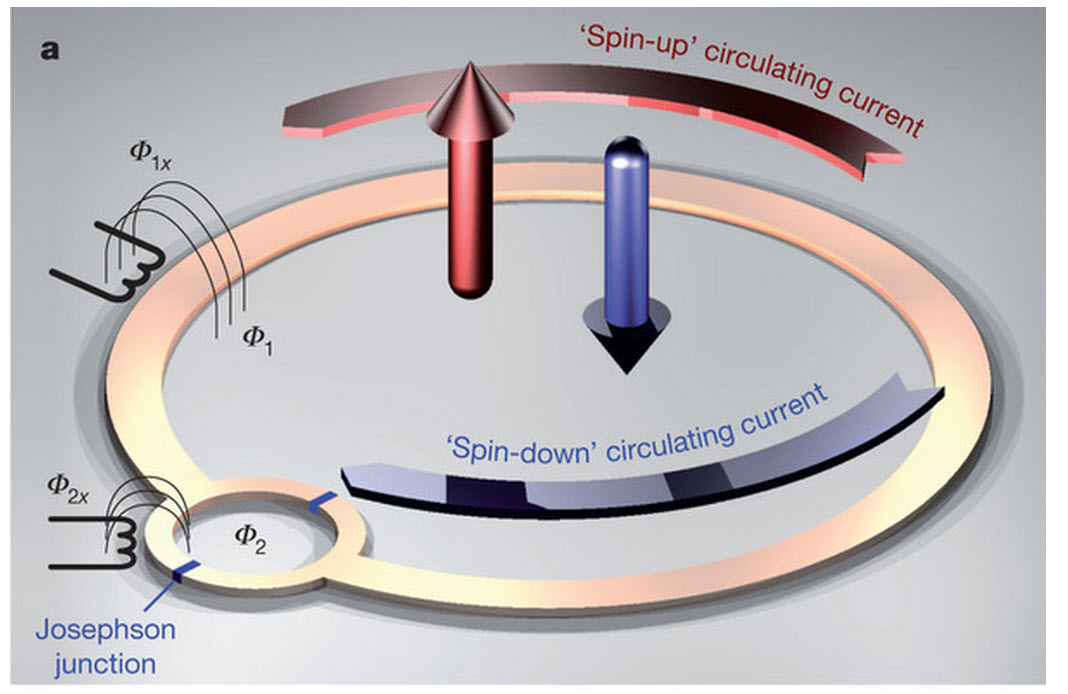
\includegraphics[scale=.25]{pasted15}
    \end{minipage}%
\end{figure}


\end{frame}

\begin{frame}{Timeline}
\begin{itemize}
  \item 1951 - EDVAC (first binary computer, Vacuum tubes)
  \item 1956 - John Bardeen invents the transistor
  \item 1958 - Jack Kilby invents ICs
  \item 1964 - IBM System/360
  \item 1968 - Intel founded by Robert Noyce
  \item 1971 - Intel 4004 (first commercially available processor, 4bit @ 740 kHz)
  \item 1975 - MITS Altair 8800 (first commercially successful hobby computer @ \$397 $\approx$ \$1700, uses Intel 8080) 
\end{itemize}
\end{frame}






\begin{frame}{Appendix $U_f$}

\begin{eqnarray*}
U_{f}\left(\Ket{x}\left(\frac{\Ket{0}-\Ket{1}}{\sqrt{2}}\right)\right)	&=	U_{f}\left(\frac{\Ket{x}\Ket{0}-\Ket{x}\Ket{1}}{\sqrt{2}}\right)\\
&=	\frac{\Ket{x}\Ket{0\oplus f\left(x\right)}-\Ket{x}\Ket{1\oplus f\left(x\right)}}{\sqrt{2}}
\end{eqnarray*}

Now if $f\left(x\right)=0$ then 
\[
\frac{\Ket{x}\Ket{0\oplus f\left(x\right)}-\Ket{x}\Ket{1\oplus f\left(x\right)}}{\sqrt{2}}=\frac{\Ket{x}\Ket{0}-\Ket{x}\Ket{1}}{\sqrt{2}}
\]

and if $f\left(x\right)=1$ then because $\oplus$ is mod 2 
\[
\frac{\Ket{x}\Ket{0\oplus f\left(x\right)}-\Ket{x}\Ket{1\oplus f\left(x\right)}}{\sqrt{2}}=\frac{\Ket{x}\Ket{1}-\Ket{x}\Ket{0}}{\sqrt{2}}
\]


\end{frame}
\begin{frame}{Appendix $U_f$}
and so
\begin{eqnarray*}
U_{f}\left(\Ket{x}\left(\frac{\Ket{0}-\Ket{1}}{\sqrt{2}}\right)\right)	&=	U_{f}\left(\frac{\Ket{x}\Ket{0}-\Ket{x}\Ket{1}}{\sqrt{2}}\right)\\
	&=	\frac{\Ket{x}\Ket{0\oplus f\left(x\right)}-\Ket{x}\Ket{1\oplus f\left(x\right)}}{\sqrt{2}}
\end{eqnarray*}

Succintly put 
\[
U_{f}\left(\Ket{x}\left(\frac{\Ket{0}-\Ket{1}}{\sqrt{2}}\right)\right)	=	\left(-1\right)^{f\left(x\right)}\Ket{x}\left(\frac{\Ket{0}-\Ket{1}}{\sqrt{2}}\right)
\]
\end{frame}
\begin{frame}{Appendix Deutsch}

\begin{eqnarray*}
\Ket{\psi_{1}} & = & H^{\otimes2}\left(\Ket{0}\otimes\Ket{1}\right)\\
 & = & \left(H\Ket{0}\right)\otimes\left(H\Ket{1}\right)\\
 & = & \left(\frac{1}{\sqrt{2}}\left(\Ket{0}+\Ket{1}\right)\right)\otimes\left(\frac{1}{\sqrt{2}}\left(\Ket{0}-\Ket{1}\right)\right)\\
 & = & \Ket{0}\otimes\frac{\Ket{0}-\Ket{1}}{\sqrt{2}}+\Ket{1}\otimes\left(\frac{\Ket{0}-\Ket{1}}{\sqrt{2}}\right)
\end{eqnarray*}
Then 
\[
\psi_{2}=U_{f}\Ket{\psi_{1}}=\begin{cases}
\pm & \left(\frac{\Ket{0}+\Ket{1}}{\sqrt{2}}\right)\left(\frac{\Ket{0}-\Ket{1}}{\sqrt{2}}\right)\text{ if }f\left(0\right)=f\left(1\right)\\
\pm & \left(\frac{\Ket{0}-\Ket{1}}{\sqrt{2}}\right)\left(\frac{\Ket{0}-\Ket{1}}{\sqrt{2}}\right)\text{ if }f\left(0\right)\neq f\left(1\right)
\end{cases}
\]
The final Hadamard gate on the first qubit gives
\[
\psi_{3}=\begin{cases}
\pm & \Ket{0}\left(\frac{\Ket{0}-\Ket{1}}{\sqrt{2}}\right)\text{ if }f\left(0\right)=f\left(1\right)\\
\pm & \Ket{1}\left(\frac{\Ket{0}-\Ket{1}}{\sqrt{2}}\right)\text{ if }f\left(0\right)\neq f\left(1\right)
\end{cases}
\]
\end{frame}

\begin{frame}{Appendix Josza}
\[
\psi_{2}=U_{f}\psi_{1}=\sum_{x\in\left\{ 0,1\right\} ^{n}}\frac{\left(-1\right)^{f\left(x\right)}\Ket{x}}{\sqrt{2^{n}}}\left(\frac{\Ket{0}-\Ket{1}}{\sqrt{2}}\right)
\]
Now extrapolating from $H\Ket{0}=\sum_{z\in\left\{ 0,1\right\} }\left(-1\right)^{0\cdot z}\Ket{z}/\sqrt{2}$
and $H\Ket{1}=\sum_{z\in\left\{ 0,1\right\} }\left(-1\right)^{1\cdot z}\Ket{z}/\sqrt{2}$ applying
to 
\begin{eqnarray*}
H^{\otimes n}\Ket{x_{1},\dots,x_{n}}_{x_{i}\in\left\{ 0,1\right\} } & = & \bigotimes_{i=1}^{n}\left(H\Ket{x_{i}}\right)_{x_{i}\in\left\{ 0,1\right\} }\\
 & = & \left(\sum_{z\in\left\{ 0,1\right\} }\frac{\left(-1\right)^{x_{i}\cdot z}}{\sqrt{2}}\Ket{z}\right)_{x_{i}\in\left\{ 0,1\right\} }^{\otimes n}\\
 & = & \sum_{z_{1},\dots,z_{n}}\frac{\left(-1\right)^{x_{1}z_{1}+\cdots+x_{n}z_{n}}}{\sqrt{2^{n}}}\Ket{z_{1},\dots,z_{n}}
\end{eqnarray*}
\end{frame}


\begin{frame}[allowframebreaks]{Bibliography}
\bibliography{tof.bib} 
\end{frame}
\end{document}


